\documentclass[spanish, 12pt,a4paper]{article}
%\usepackage[spanish]{babel}
\usepackage{algorithmic}
%\usepackage{savesym}
%\savesymbol{IF, algorithmic}
\usepackage[utf8]{inputenc}
\usepackage[spanish]{babel}
\usepackage{aed2-symb}
\usepackage{textcomp}
\usepackage[section, ruled]{algorithm}
\usepackage{hyperref}
\usepackage[pdftex]{graphicx}
\usepackage{epsfig}

\floatname{algorithm}{Algoritmo} % para que diga ``Algoritmo'' y no ``Algorithm''

\renewcommand{\algorithmiccomment}[1]{\ \ \ \textbf{//#1}} %para agregar comntarios en los algoritmos poner
% \COMMENT{ALAN ES GAY}
% \usepackage{algpseudocode}
% \usepackage{lineno}
\newenvironment{parr}
{\begin{list}{}%
         {\setlength{\leftmargin}{2em}}%
         \item[]%
}
{\end{list}}
\newcommand{\tab}{\hspace*{2em}}

\newcommand{\oper}[3]{\samepage\textsc{#1}(#2) $\rightarrow$ \textit{res} $\colon$ #3\\*}
\newcommand{\operL}[3]{\samepage\textsc{#1}(#2) $\rightarrow$ \textit{res} $\colon$ #3}
\newcommand{\operM}[2]{\samepage\textsc{#1}(#2)\\} %�sta es la operaci�n que no devuelve nada
\newcommand{\operMA}[2]{\samepage\textsc{#1}(#2)} %�sta es la operaci�n que no devuelve nada y para usar en el
%``caption'' del ``algorithm''
\newcommand{\vin}[2]{\textbf{in} \textit{#1}$\colon$#2}
\newcommand{\vinout}[2]{\textbf{in/out} \textit{#1}$\colon$#2}
\newcommand{\pre}[1]{\textbf{Pre} $\equiv$ \{#1\}\\*}
\newcommand{\post}[1]{\textbf{Post} $\equiv$ \{#1\}\\*}
\newcommand{\complej}[1]{\textbf{Complejidad:} #1\\*}
\newcommand{\desc}[1]{\textbf{Descripci\'on:} #1\\}
\newcommand{\alias}[1]{\textbf{Aliasing:} #1\\}

% \oper{nombre}{recibe}{devuelve}
% \vin{var}{tipo}
% \vinout{var}{tipo}
% \pre{}
% \post{}
% \complej{O()}
% \desc{txt}
% \alias{txt}

\newcommand{\eqobs}{$=_{obs}$}
\newcommand{\bigo}[1]{O$\big($#1$\big)$}
\newcommand{\NULL}{\textsc{Null} }
\newcommand{\aux}[3]{\samepage #1$\colon$ #2 $\rightarrow$ #3\\*}

\usepackage{hyperref}
\usepackage{color}
\usepackage{graphicx}
\usepackage{graphics}
\usepackage{clrscode3e}
\usepackage{amsthm}
\usepackage{caption}
\usepackage{subcaption}
\usepackage{caratula}
\usepackage{fancyhdr,lastpage}
\usepackage[paper=a4paper, left=1.4cm, right=1.4cm, bottom=1.4cm, top=1.4cm]{geometry}
\usepackage[table]{xcolor} % color en las matrices
\usepackage[font=small,labelfont=bf]{caption} % caption de las figuras en letra mas chica que el texto
  
\color{black}

%%%PAGE LAYOUT%%%
\topmargin = -0.5cm
\voffset = 0cm
\hoffset = 0em
\textwidth = 37em
\textheight = 130 ex
\oddsidemargin = 4 em
\parindent = 2 em
\parskip = 3 pt
\footskip = 7ex
\headheight = 20pt
\pagestyle{fancy}
\lhead{AyED	 III - 2013 C1 - Trabajo Pr\'actico 2} % cambia la parte izquierda del encabezado
\renewcommand{\sectionmark}[1]{\markboth{#1}{}} % cambia la parte derecha del encabezado
\rfoot{\thepage}
\cfoot{}
\numberwithin{equation}{section} %sets equation numbers <chapter>.<section>.<subsection>.<index>

%Lo siguiente controla el ancho de las figuras (principalmente para el texto de los captions)
%\newcommand{\figurewidth}{.9\textwidth}
\newcommand{\figurewidth}{1\textwidth}

\newcommand{\tuple}[1]{\ensuremath{\left \langle #1 \right \rangle }}
\newcommand{\Ode}[1]{\small{$\mathcal{O}(#1)$}}
\newtheorem{teorema}{Teorema}[section]


%El siguiente paquete permite escribir la caratula facilmente
\hypersetup{
  pdftitle={ Algoritmos III - TP1 },
  colorlinks,
  citecolor=black,
  filecolor=black,
  linkcolor=black,
  urlcolor=black 
}

\materia{Algoritmos y Estructuras de Datos III}

\titulo{Trabajo Práctico 1}

\subtitulo{Informe y análisis de resultados.}

%\grupo{Grupo 8}
 
\integrante{Benitti, Raul}{592/08}{raulbenitti@gmail.com}
\integrante{Mengarda,Lucas }{}{l.j.mengarda@gmail.com}
\integrante{Scarpino, Gino}{392/08}{gino.scarpino@gmail.com}
\integrante{Vallejo, Nicolás}{}{nico\_pr08@hotmail.com}
 
\begin{document}
{ \oddsidemargin = 1em
	\headheight = -20pt
	\maketitle
}
	\tableofcontents
	\newpage
%	\section*{Introducción}
\addcontentsline{toc}{section}{Introducci\'on}

En el presente trabajo práctico se intenta resolver ciertos problemas brindados por la c\'atedra, 
por medio de algoritmos que resuelvan dichos problemas. Se decidi\'o implementar dichas soluciones 
usando el lenguaje \textit{Java} y \textit{C++}. Junto con las implementaciones, se adjunta un 
informe que especifica los detalles sobre el desarrollo de las soluciones, as\'i como pruebas, 
cálculos de complejidad temporal, mediciones, etc.\\
Cabe aclarar, que dada la naturaleza de los problemas planteados, se decidi\'o calcular y 
expresar la complejidad de los algoritmos involucrados, usando el \textbf{modelo de costos uniforme}.

%	\newpage
	\section{Problema 1: Mutaciones bacteriales}
 
\subsection{Introducci\'on}

El estudio de las mutaciones bacteriales es un trabajo arduo y pesado. 
Una bacteria, al nacer, pertenece a una cepa determinada. 
Con el tiempo, la bacteria va mutando de una cepa a otra hasta que en
alg\'un momento alcanza una cepa terminal desde la cual yo no puede seguir mutando. 
Durante el proceso, estando en una cierta cepa, la bacteria puede mutar hacia algunas otras cepas con una cierta probabilidad;
es decir, no desde cualquier cepa puede mutarse directamente a cualquier otra. 
Afortunadamente, las posibles mutaciones a partir de cada cepa son datos conocidos.
Sin embargo, no se sabe
a priori cu\'anto puede tardar una bacteria en llegar a su estado final. 
Adem\'as, en funci\'on de las posibles mutaciones entre cepas, podr\'ia darse el caso de
que una bacteria que nunca alcance un estado terminal.

Como antecedente para realizar un estudio estad\'istico de este comportamiento, en el cual se estudiar\'an algunas bacterias y para cada una de ellas se registrar\'a cada mutaci\'on ocurrida desde su nacimiento hasta que la misma deja de mutar, se desea predecir si toda sucesi\'on de mutaciones llega a un estado final, y en los casos en los que esto suceda, calcular la sucesi\'on de mutaciones de mayor longitud por la que una bacteria puede
pasar. 

\subsection{Desarrollo}

Comenzamos modelando el escenario del problema como un grafo dirigido (digrafo) donde cada nodo representa una cepa, y cada arista, la mutación de una cepa origen a una cepa destino. 
As\'i, una secuencia de mutaciones equivale a un camino en el digrafo. 
Adem\'as, si el digrafo presenta un ciclo, entonces podemos deducir que existe la posibilidad de que una bacteria nunca alcance una cepa terminal.
Por lo tanto, para resolver el problema planteado, en primer lugar necesitaremos decidir si el digrafo generado es un digrafo ac\'iclico (DAG), y en caso de serlo, encontrar la secuencia m\'as larga de mutaciones equivaldr\'a a hallar el camino (necesariamente simple) m\'as largo dentro de dicho DAG.

Trataremos primero el problema de encontrar el camino simple m\'as largo dentro de un digrafo, suponiendo que este es ac\'iclico. 
Empecemos entonces pensando en como encontrar el camino simple m\'as largo con origen en un nodo cualquiera.
Supongamos que partimos del nodo A. 
El camino m\'as largo que podemos hallar desde A a cualquier otro nodo en el DAG necesariamente
debe pasar por alguno de los nodos sucesores de A. Sea B el nodo sucesor de A tal que el camino m\'as largo con inicio en B es el mayor entre los caminos con inicio en algun nodo sucesor de A:
el camino m\'as largo a partir de A debe ser el camino m\'as largo a partir de B, m\'as la arista que une a A con B.

Esta idea revela una subestructura \'optima sobre la cual tratar el problema (en la secci\'on de Correctiud revisaremos esto). Por otro lado, como varios nodos pueden compartir sucesores, se produce un solapamiento de los subproblemas a resolver.  
Esto nos lleva naturalmente a pensar en aplicar la t\'ecnica de programaci\'on din\'amica en la resoluci\'on del problema.

Definamos, entonces, dado G=(V, E) un DAG, la funci\'on recursiva $F(v)$ como la longitud del camino simple más largo que comienza en el nodo $v$, 

$$F(v)= \max_{(v, u)\;\in\;E} \{F(u)\; + \; 1\}$$

En esta definici\'on consideramos que el m\'aximo de un conjunto vac\'io es 0.

En lugar de implementar una funci\'on recursiva (inmediata a partir de la definici\'on de F), nos centraemos directamente en un
algoritmo iterativo. 
Para esto, debemos entender en que orden debemos resolver los subproblemas, de manera de tener los datos necesarios ya calculados al momento de necesitarlos. 
De la definici\'on de F podemos ver que, al calcular la soluci\'on para un nodo i, solo necesitamos tener las subsoluciones de sus nodos sucesores. 
Para lograr esto, podemos proceder calculando las subsoluciones de los nodos seg\'un un ordenamiento topol\'ogico invertido (es decir, un ordenamiento topol\'ogico recorrido de derecha a izquierda).
Un ordenamiento topol\'ogico de los nodos de un digrafo es aquel en el que ning\'un nodo sucesor aparece antes que su predecesor (es decir, si un digrafo G contiene un eje (u, v), entonces u aparece antes que v en el ordenamiento [Cormen]). Notemos que un digrafo tiene ordenamiento topol\'ogico si y solo si es ac\'iclico, y que este ordenamiento no siempre es único. Por lo tanto, siguiendo el orden propuesto, primero calcularemos los nodos que no tienen sucesores, luego los que tiene como sucesores a los primeros, y as\'i sucesivamente hasta llegar a los nodos que no tienen antecesores.

El algoritmo iterativo de programaci\'on din\'amica mantendr\'a un arreglo $L$, tal que $L[i]$ represente la longitud del camino simple mas largo que nace en el nodo $i$, y lo llenaremos siguiendo el ordenamiento previamente explicado. 
Adem\'as, mantendremos un arreglo $S$, donde $S[i]$ es es el nodo hijo de $i$ que se eligi\'o como subsoluci\'on \'optima al problema de encontrar el camino m\'as largo desde $i$. De esta manera, al terminar el llenado de los arreglos podremos reconstuir el camino simple de mayor longitud que parte de cada nodo.

Calcularemos el ordenamiento topol\'ogico del digrafo siguiendo la idea planteada en [Cormen], el cual propone la utilizaci\'on del algoritmo de recorrido \textbf{DFS} (Depth First Search o búsqueda en profundidad). 
Una ventaja de dicho algoritmo es que procesa digrafo conexos y no conexos sin necesitar hacer distinci\'on, por lo que quedamos exentos de tener decidir si los datos de entrada generan un digrafo de un tipo o del otro. 
Dado que durante la corrida de DFS un nodo $v$ que est\'a siendo explorado aparecer\'a como vecino de alg\'un sucesor $w$ (es decir, $w$ tiene un $back-edge$ a $v$) solo si existe un ciclo, incluimos una verificaci\'on que implica el corte de la ejecuci\'on si un ciclo es detectado, y no afecta al resto de la l\'ogica.
De esta forma, en un \'unico paso inicial decidimos si el digrafo es ac\'iclico mientras que obtenemos la informaci\'on necesaria para proceder con el algoritmo de programaci\'on din\'amica. 

Ahora volvamos al problema original. 
Usando el algoritmo previamente explicado, podemos calcular, para cada nodo $v$, el camino simple m\'as largo que tiene a $v$ como origen.
%Observemos que, de entre todos estos caminos, el de mayor longitud deber\'a tener como primer nodo a alg\'un nodo del DAG cuyo grado de entrada sea cero, y como \'ultimo nodo, alguno cuyo grado de salida sea cero. 
%Para demostrar esto, supongamos un camino simple $C = v_i...v_j$ de longitud m\'axima $n$. 
%Por un lado, si el grado de entrada de $v_i$ es distinto de cero, entonces debe existir alg\'un otro nodo $v_{i-1}$ tal que $v_{i-1}$ no se encuentra en $C$ (por ser el grafo un DAG) y $v_{i-1}$$v_i$ es una arista del digrafo analizado. 
%Pero, siendo este el caso, podr\'iamos agregar tal arista al camino $C$, obteniendo un camino $C' = v_{i-1}v_i...v_j$ de mayor longitud que $C$, lo cual es absurdo pues supusimo $C$ un camino simple de longitud m\'axima.    
%Por otro lado, si el grado de salida de $v_{j}$ es distinto de cero, entonces debe existir alg\'un otro nodo $v_{j+1}$ tal que $v_{j+1}$ no se encuentra en $C$ (por ser el grafo un DAG) y $v_{j}$$v_{j+1}$ es una arista del digrafo analizado. De nuevo, si este el caso, podr\'iamos agregar tal arista al camino $C$, obteniendo un camino $C' = v_i...v_jv_{j+1}$ de mayor longitud que $C$, lo cual es absurdo pues supusimo $C$ un camino simple de longitud m\'axima.
Se desprende que el camino m\'as largo ser\'a el m\'ayor de todas estas soluciones. En el caso en que exista m\'as de un candidato, devolveremos aquel camino que comience en el nodo de menor \'indice. 



\subsection{Algoritmo}
Como ya mencionamos, el algoritmo para generar el orden topol\'ogico est\'a explicado en [Cormen, p603-614]
Las funciones $ordenTopologico$ y $visitar$ consideran a un nodo de la siguiente manera:
ABIERTO, si todavía no se fue visitado; 
DESCUBIERTO, si se lo ha visitado pero todavía no se recorrieron todos sus vecinos;
CERRADO, una vez que se recorrió todos sus vecinos.

Antes de llamar a $ordenTopologico$ todos los nodos son marcados como ABIERTO. 


\begin{algorithm}[H]
\caption{} 
\label{pseudocodigo_ordenTopologico}
\begin{codebox}
\Procname{$\proc{ordenTopologico}(grafo$ G$)$}
\li \While existe nodo ABIERTO en G\Do
\li		n $\gets$ seleccionar nodo ABIERTO
\li		\If visitar(n, nodosOrdenados) igual a HAY CICLO 	\Do 
\li				\Return HAY CICLO
			\End
		\End
\li	\Return nodosOrdenados	  
	\End
\end{codebox}
\end{algorithm}


\begin{algorithm}[H]
\caption{} 
\begin{codebox}
\Procname{$\proc{visitar}(nodo$ n, $lista$ nodosOrdenados$)$}
\li \Comment{El siguiente If es la unica modificacion al algoritmo de Cormen}	
\li \If n es DESCUBIERTO \Do
\li 	 \Return HAY CICLO
 		\End
\li \If n es ABIERTO \Do
\li 	marcar n como DESCUBIERTO
\li		\For cada m sucesor de n \Do
\li			visitar(m)			
			\End	
\li		marcar n como CERRADO
\li 		insertar n al principio de $nodosOrdenados$
\li 	\Return
 		\End
	\End
\end{codebox}
\end{algorithm}
 

\begin{algorithm}[H]
\caption{} 
\label{pseudocodigo_caminoMaximo}
\begin{codebox}
\Procname{$\proc{caminoMaximo}(digrafo$ G$)$}
\li \Comment{ Verificar si hay ciclo en G y obtener orden topologico de sus nodos, si es posible}
\li orden $\gets$ ordentTopologico
\li \If orden es un orden topologico valido (no hay ciclo) \Do
\li		\For cada nodo v en orden invertido\Do
\li			L[v] $\gets$ 0
\li 		S[v] $\gets$ 0
\li			\For cada w sucesor de v \Do
\li		  	\If L[w] + 1 $>$ L[v] \Do
\li				L[v] $\gets$ L[w]+ 1
\li				S[v] $\gets$ w
					\End
				\End
			\End
\li 	camino $\gets$ armarCamino(L, S)
\li 	\Return longitud(camino), camino
		\End
\li \Else \Do
\li 	\Return -1
		\End
	\End
\end{codebox}
\end{algorithm}


\begin{algorithm}[H]
\caption{} 
\label{pseudocodigo_armarCamino}
\begin{codebox}
\Procname{$\proc{armarCamino}(lista$ L , $lista$ S)}
\li camino $\gets$ lista vacia
\li v $\gets$ indice maximo valor en L
\li Agregar v al fin de camino 
\li	\While S[v] distinto de 0 \Do
\li		v $\gets$ S[v]
\li		Agregar v al fin de camino
	\End
\li \Return camino	
	\End
\end{codebox}
\end{algorithm}

\subsubsection{Correctitud} 

Dijimos que el problema presenta un subestructura \'optima. Para ver esto, observemos que la soluci\'on se basa en subsoluciones a subproblemas de igual tipo pero menor tama\~no. 
Podemos afirmar que los tama\~nos de las subinstancias ser\'an menores porque, dado que estamos trabajando sobre un DAG, al tratar de encontrar el camino m\'aximo desde los nodos sucesores de A sabemos que no podemos volver a pasar por A o alguno de sus predecesores puesto que esto implicar\'ia tener un ciclo, lo que no es posible por definici\'on. 
Adem\'as, las subsoluciones deben ser \'optimas: supongamos que tenemos una soluci\'on \'optima que usa una subsoluci\'on no \'optima de un subproblema dado (y que a\'un as\'i la soluci\'on de este subproblema resulta ser la mejor elecci\'on entre las subsoluciones consideradas). Supongamos adem\'as que conocemos una subsoluci\'on \'optima, de manera que el largo de este camino es estrictamente mayor que el de la subsoluci\'on usada. Si reemplazamos, en la soluci\'on, la subsoluci\'on no \'optima por la nueva subsoluci\'on \'optima, entonces obtendremos un camino de mayor longitud que el \'optimo, lo que es absurdo.

Veamos ahora que el algoritmo propuesto calcula el camino m\'as largo. 
Para esto, debemos mostrar que, al finalizar,  el ciclo de las lineas 4 a 10 del Algoritmo \ref{pseudocodigo_caminoMaximo} carga los arreglos $L$ y $S$ de manera que $L[v]$ es la longitud del camino simple m\'as largo desde $v$ a cualquier otro nodo $w$, y que el recorrido generado siguiendo los ejes $(v, S[v])$ (mientras que $S[v]$ est\'e definido) es dicho camino simple. 
Si $v$ no tiene sucesores, entonces no existen caminos de v a ning\'un otro nodo. 
Por lo tanto, $L[v] = 0 = F(v)$ es el valor correcto y no se considera niguna arista ( $(v, S[v]) = (v, indefinido)$ no es un eje existente). 
Si $v$ tiene sucesores, supongamos que los valores de L para estos son correctos (es decir, si $(v, w) \in  E(G)$ entonces $L[w] = F(w)$):
dado que vamos calculando L siguiendo un ordenamiento topol\'ogico le\'ido de derecha a izquierda, los valores de L para los sucesores de v ya habr\'an sido calculados al momento de llegar a $v$. 
Como ya vimos, para llegar a cualquier nodo alcanzable desde $v$ debemos pasar por alguno de los sucesores de $v$.  Entonces, la distancia maxima de $v$ a cualquier otro nodo depende de la distancia m\'axima de sus sucesores a cualquier otro nodo: en el algoritmo, el subciclo de las lineas 7-10 elige el sucesor $w$ con mayor $L[w]$ y se guarda $w$ en $S[v]$. Asi, $L[v] = \max_{(v,w) \in E(G)}{L[w]+1} = \max_{(v,w) \in E(G)}{F(w) +1} = F(v) $
El recorrido $vS[v]S[S[v]]...S[...S[v]]...0$ es un camino simple, pues al ser el digrafo ac\'iclico, ning\'un nodo puede tener como sucesor a alguno de los anteriores.


\subsubsection{An\'alisis de complejidad}
 
El Algoritmo \ref{pseudocodigo_ordenTopologico}, al ser \textbf{DFS}, tiene orden O($\left|{E}\right|$+$\left|{V}\right|$).
El Algoritmo \ref{pseudocodigo_armarCamino} recorre un arreglo con O($\left|{V}\right|$) posiciones, y dado que se asume que no existen ciclos, a lo sumo pasa una vez por cada posici\'on. Por lo tanto, es del orden O$\left|{V}\right|$).
En el Algoritmo \ref{pseudocodigo_caminoMaximo} se recorren todos los nodos del grafo una \'unica vez (en el ciclo de las l\'ineas 4-12), y por cada uno, se recorren todas sus aristas tambien una \'unica vez (en el ciclo de las l\'ineas 7-10), por lo que el el ciclo mayor tiene complejidad en el orden de O($\left|{E}\right|$+$\left|{V}\right|$). Adem\'as, se llama a cada una de las dos funciones previamente mencionadas una \'unica vez: en total, la complejidad del algoritmo resulta en el orden de O($\left|{E}\right|$+$\left|{V}\right|$).
 

\subsection{Pruebas}
Para las pruebas de correctitud utilizamos grafos peque\~nos que pueden resolverse f\'acilmente a mano. 
Los casos que elegimos fueron digrafos con ciclos y sin ciclos, tanto de una \'unica componente conexa como m\'as de una.


Para probar la performance del algoritmo, armamos casos de digrafos aleatorios (que pueden o no contener ciclos) y DAGs. Probamos casos separados por n\'umero de nodos fijos (sobre los que variamos la cantidad de aristas) y n\'umero de aristas fijo (donde variamos la cantidad de nodos). 
No encontramos familias de casos que tuvieran un comportamiento distinto al esperado.

%%%%%%%%%%%%%%%%%%%%%%%%%%%%%%%%%%%%%%%%%%%%%%%%%%%%%%%%%%%

\begin{figure}[H]
	\centering
	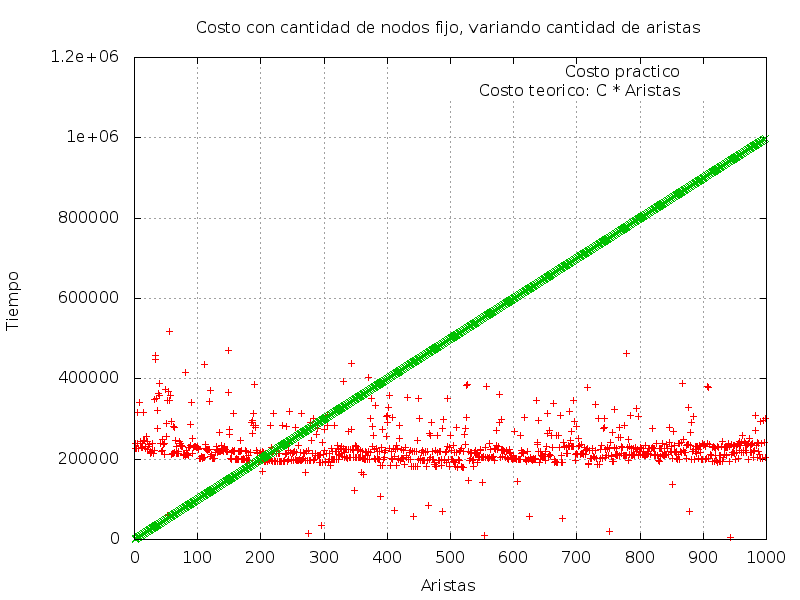
\includegraphics[scale=0.5]{dag_100.png}
	\caption{Digrafo aleatorio, n = 100, m variable}
\end{figure}

\begin{figure}[H]
	\centering
	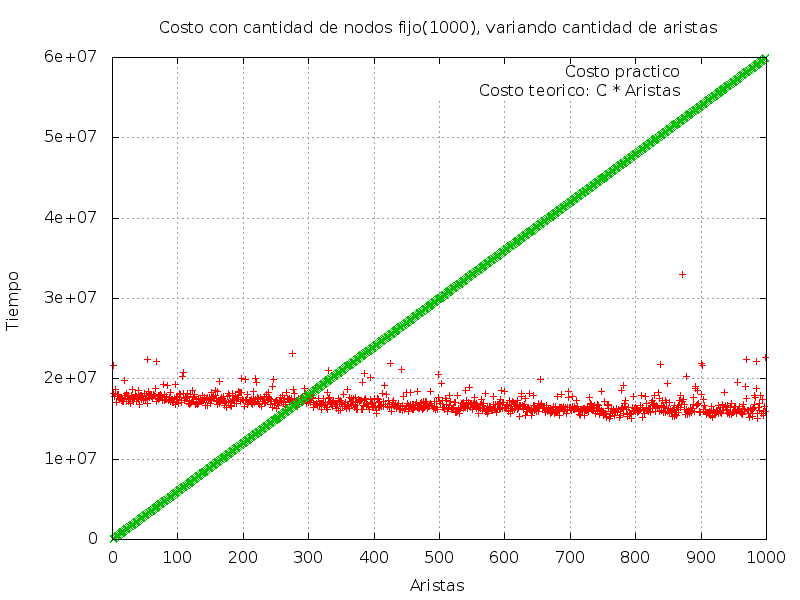
\includegraphics[scale=0.5]{dag_1000.png}
	\caption{Digrafo aleatorio, n = 1000, m variable}
\end{figure}


%%%%%%%%%%%%%%%%%%%%%%%%%%%%%%%%%%%%%%%%%%%%%%%%%%%%%%%%%%%

\begin{figure}[H]
	\centering
	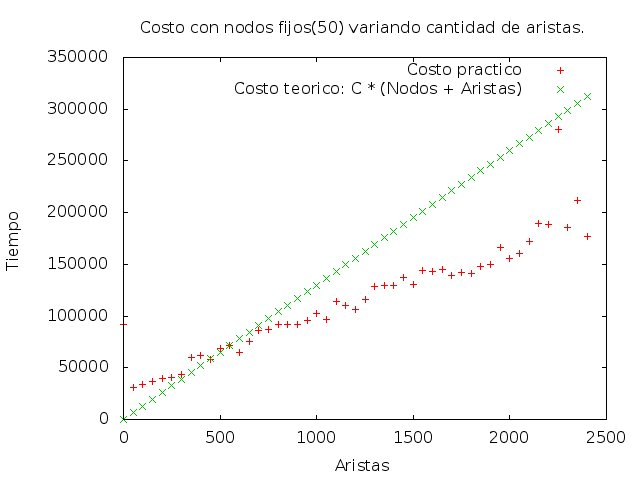
\includegraphics[scale=0.5]{blank.png}
	\caption{DAG aleatorio, n = 100, m variable}
\end{figure}

\begin{figure}[H]
	\centering
	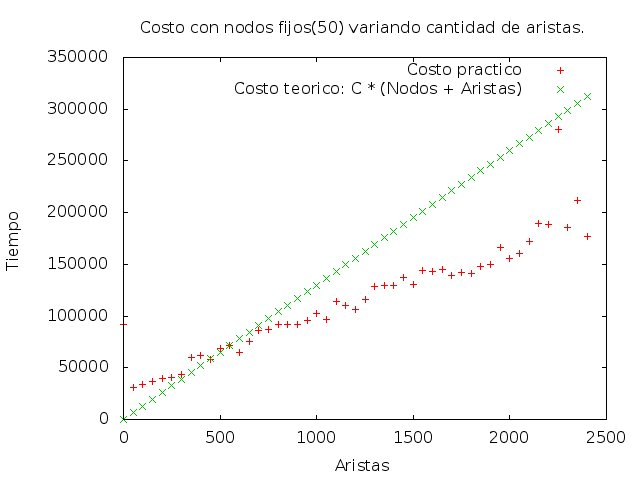
\includegraphics[scale=0.5]{blank.png}
	\caption{DAG aleatorio, n = 1000, m variable}
\end{figure}

%%%%%%%%%%%%%%%%%%%%%%%%%%%%%%%%%%%%%%%%%%%%%%%%%%%%%%%%%%%

\begin{figure}[H]
	\centering
	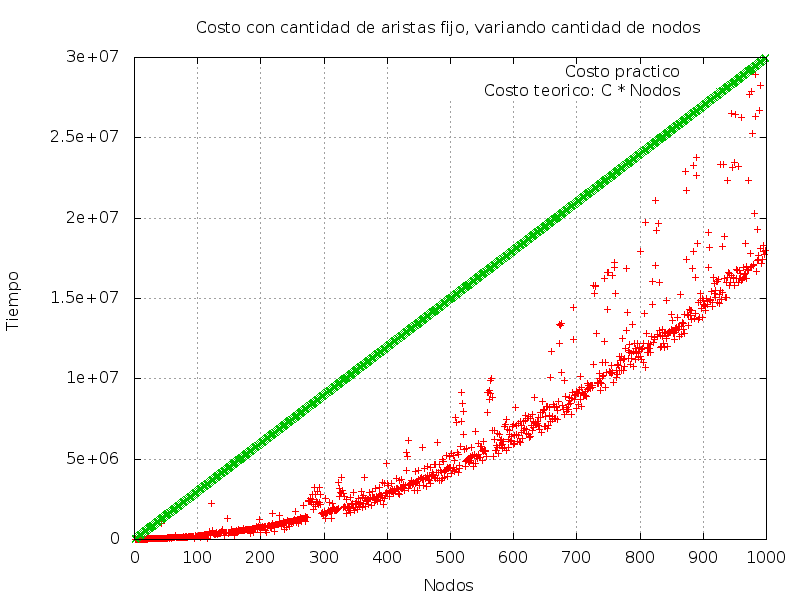
\includegraphics[scale=0.5]{dag_100_n_var.png}
	\caption{Digrafo aleatorio,  n variable, m = 100}
\end{figure}

\begin{figure}[H]
	\centering
	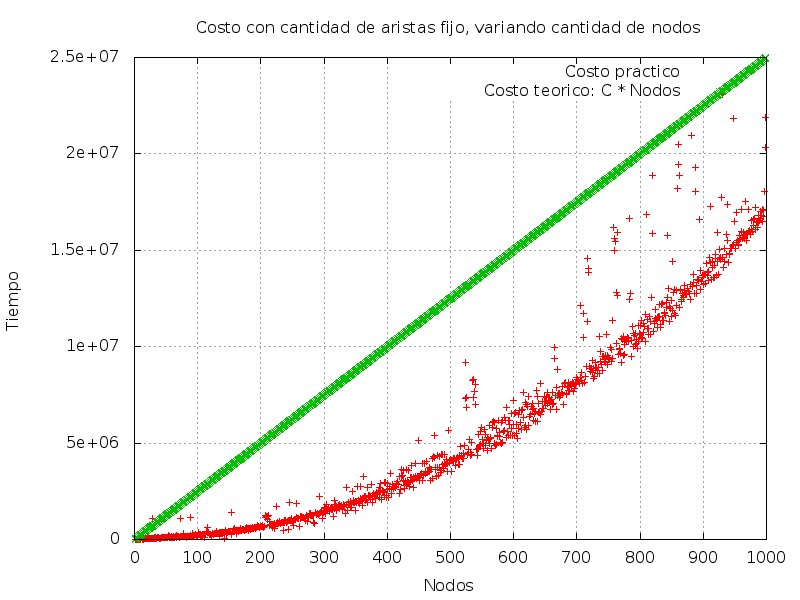
\includegraphics[scale=0.5]{dag_500_n_var.png}
	\caption{Digrafo aleatorio, n variable, m = 500}
\end{figure}



%%%%%%%%%%%%%%%%%%%%%%%%%%%%%%%%%%%%%%%%%%%%%%%%%%%%%%%%%%%

\begin{figure}[H]
	\centering
	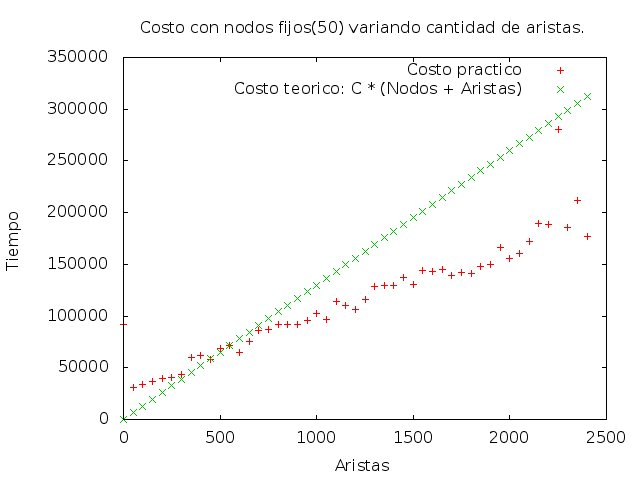
\includegraphics[scale=0.5]{blank.png}
	\caption{DAG aleatorio,  n variable, m = 100}
\end{figure}

\begin{figure}[H]
	\centering
	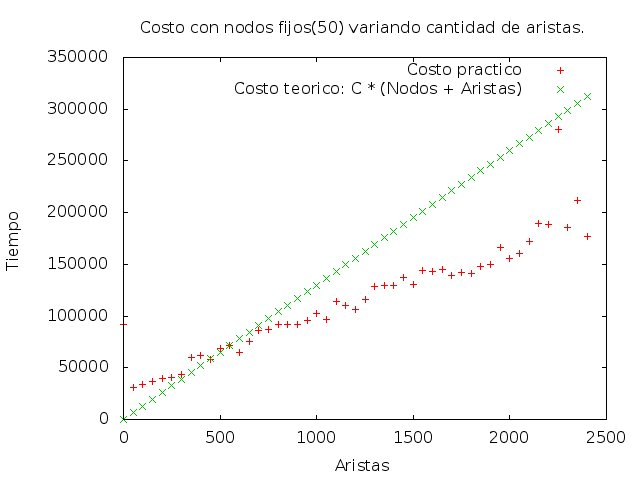
\includegraphics[scale=0.5]{blank.png}
	\caption{DAG aleatorio, n variable, m = 500}
\end{figure}


%%%%%%%%%%%%%%%%%%%%%%%%%%%%%%%%%%%%%%%%%%%%%%%%%%%%%%%%%%%

\subsection{Conclusiones}

La resoluci\'on del problema planteado en este ejercicio es un claro ejemplo de la importancia de t\'ecnicas como Programaci\'on din\'amica y algoritmos gen\'ericos sobre grafos: no solo se obtuvo un algoritmo competente en cuanto a performance (por ser de orden lineal tanto en tiempo de ejecucion como almacenaiento de datos en memoria), sino que tambien resulta ser sencillo y f\'acil de comprender.

A pesar de no estar presentes, hubiera sido interesante agregar casos de test donde variasemos la cantidad de componente conexas dejando fijas la cantidad de nodo y aristas, o la suma de ambos valores. En este caso, esperariamos que el grafico estuviera acotado por una funci\'on constante.


	\newpage
	%\section{Problema 2: Sensores defectuosos}

\subsection{Introducci\'on}

\quad Se tiene un conjunto de sensores con sus respectivos intervalos de tiempo de medici\'on y se conoce el n\'umero de la medici\'on que falla. Se desea conocer el id del sensor que fall\'o. 

\subsection{Desarrollo}

\quad Encaramos este problema rearmando la secuencia de mediciones de los sensores. Consiguiendo \'esto, la soluci\'on al problema ser\'ia fijarse en esta secuencia, el id que figura en la posici\'on de medici\'on que fall\'o.


\quad Para armar la secuencia de mediciones, decidimos ir guardando para cada sensor en que instante de tiempo tendr\'ia que volver a realizar una medici\'on. A medida que determinamos el sensor que va a medir, calculamos su siguiente tiempo de medici\'on.


\quad Teniendo un diccionario donde para cada sensor se puede obtener en qu\'e momento le toca realizar una medici\'on, se puede conocer al pr\'oximo que le toca medir, ya que es el m\'inimo de los tiempos.


\quad En el momento inicial todos los sensores miden, por lo que la secuencia inicial no es vac\'ia, sino que contiene todos los n\'umeros de sensores ordenados por su id ya que desempatan por \'este.


\quad En cada paso de nuestro algoritmo, agregamos a la secuencia el siguiente sensor que midi\'o y calculamos su pr\'oxima medici\'on actualizando la tabla de pr\'oximas mediciones


\quad Cuando la secuencia alcanza el tama\~no igual al n\'umero de medici\'on que fall\'o, terminamos y el resultado es la \'ultima posici\'on de esa secuencia.

\quad

\textbf{Aclaraci\'on:} en la implementaci\'on del diccionario se usa directamente un min-Heap. M\'as adelante se explica el motivo de tal decisi\'on.



\quad


\textbf{Pseudoc\'odigo:}

\begin{algorithm}[H]
\begin{algorithmic}[1]
\STATE Diccionario diccTiempos  \quad $ \gets $ \quad sensores
\STATE Entero medicion $ \gets \vert$ sensores $ \vert $
\FORALL{ Sensor s \textbf{in} sensores}
\STATE agregar(mediciones,id(s))
\ENDFOR
\WHILE{medicion < medDefectuosa}
\STATE proximo \quad $ \gets $ \quad proxSensor(diccTiempos,sensores)
\STATE agregar(mediciones,proximo)
\STATE medicion $ \gets $ medicion + 1
\ENDWHILE
\end{algorithmic}
\caption{Entero sensorDefectuoso(Conjunto sensores, Entero medDefectuosa)}\label{probConjK}
\end{algorithm}


\quad


\textbf{Donde}


\quad \quad \quad medDefectuosa es el n\'umero de medici\'on que falla.

\quad


\quad \quad \quad diccTiempos es el diccionario que para cada sensor guarda el tiempo de su pr\'oxima medici\'on.

\quad


\quad \quad \quad sensores es el conjunto de sensores.


\quad

\quad \quad \quad medicion es el n\'umero de medici\'on parcial. Como al inicio hubo la cantidad de sensores, se inicializa con esa cantidad.


\quad

\quad \quad \quad mediciones es la secuencia de mediciones con los ids de los sensores.


\quad

\quad \quad \quad proxSensor es la funcion que devuelve el id del m\'inimo de los tiempos que est\'an presentes en el diccionario, y adem\'as actualiza el tiempo para la pr\'oxima medici\'on.


\subsubsection{Correctitud}

\quad En alguna instancia del problema, si tuvi\'eramos la siguiente tabla con los momentos $ t_i $ para la siguiente medici\'on de cada sensor $ s_i $ con \quad  $ (1 \leq i \leq n)$ \quad donde n es la cantidad total de sensores:


\quad


\begin{tabular}{| c | c | c | c | c |}
\hline
$ s_1 $ & $ s_2 $ & ... & $ s_{n-1} $ & $ s_n $\\
\hline
$ t_1 $ & $ t_2 $ & ... & $ t_{n-1} $ & $ t_n $\\
\hline

\end{tabular}



\quad


\quad determinar el siguiente sensor que le toca realizar su medici\'on, ser\'ia elegir el de menor t. Caso contrario, se estar\'ia eligiendo un sensor con tiempo mayor, por lo que har\'ia una medici\'on anterior cuando en realidad le corresponder\'ia a un sensor con menos tiempo, generando una incongruencia en el orden de mediciones.

\quad Por lo que alcanzar\'ia con ver que nuestro algoritmo genera esa tabla/diccionario de forma correcta.

\quad En el instante inicial, el diccionario contendr\'a los tiempos de intervalos de medici\'on ya que todos midieron de entrada. Para el primero, elegimos el m\'inimo de esos tiempos. Una vez que sabemos el id, lo agregamos a la secuencia de mediciones, y redefinimos en el diccionario su tiempo de la siguiente forma:


\quad


$ t'_{i} = t_{i} + intervalo(s_1) $


\quad


\quad es decir, que al tiempo que ya figuraba en el diccionario, se le agrega el tiempo de intervalo para determinar el tiempo de su pr\'oxima medici\'on. Por lo que, en cada paso donde se elige el sensor que mide, se actualiza el diccionario. De esta forma, se mantiene la correctitud del significado del diccionario una vez elegido el pr\'oximo sensor a medir.

\quad Se repite este proceso hasta llegar a la medici\'on que falla inclusive, con lo que el id del sensor quedar\'ia guardado en la secuencia de mediciones.


\subsubsection{An\'alisis de complejidad}

\quad Se cargan los datos de los sensores en vectores. En uno, el tiempo de intervalo entre mediciones. En otro, una tupla que representar\'ia la primer componente el id del sensor y la segunda componente el tiempo de pr\'oxima medici\'on. A la vez que se cargan los datos, ya se colocan los ids por orden en el vector de mediciones ya que todos miden en el instante inicial.

\quad La complejidad de lo anterior es O(n), donde n es la cantidad de sensores.

\quad En el caso que el n\'umero de medici\'on sea menor a la cantidad de sensores, el algoritmo termina devolviendo el valor del vector de mediciones seg\'un la posici\'on correspondiente a la medici\'on que falla.

\quad Caso contrario, calculamos la secuencia de mediciones. Para ello necesitamos el ya mencionado diccionario. Decidimos utilizar un min-Heap como diccionario. Esto nos permitir\'ia obtener el m\'inimo valor de tiempo de pr\'oxima medici\'on en O(log n) siendo n la cantidad de sensores. Crear el minHeap tiene un costo de O($ 3*n $).

\quad Una vez creado el minHeap, comenzamos un ciclo donde se busca el siguiente sensor que mide. Como ya dijimos, al usar un minHeap, \'esto tiene un costo de O(log n). Luego, se agrega el id del sensor a la secuencia de mediciones con un costo constante.

\quad La cantidad de iteraciones del ciclo es el n\'umero de medici\'on que falla menos la cantidad de sensores existentes. \'Esto se debe a que, en el momento inicial, todos los sensores realizan una medici\'on. Por lo que de entrada se tienen n mediciones.

\quad Por lo tanto, la complejidad total del algoritmo termina siendo:


\quad


$ \displaystyle\sum_{i = k}^{n} log n = (k - n) * log n \leq k * n$


\quad


\quad Termina siendo estrictamente menor a O($ k*n $) como se ped\'ia en la consigna.


\quad


\subsection{Resultados}

\quad Para analizar el comportamiento del nuestro algoritmo, decidimos generar un test aleatorio donde se va variando la cantidad de sensores. En el mismo nos queda una gr\'fica:


\quad


\begin{figure}[H]
	\centering
	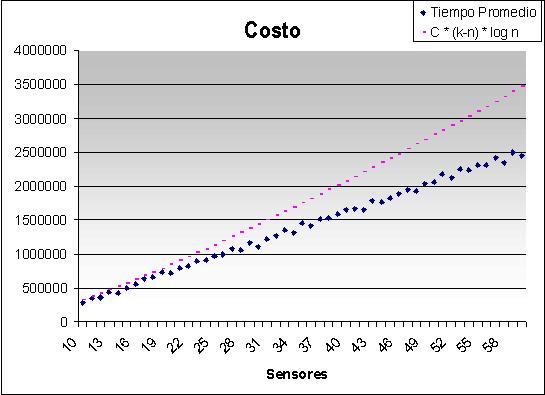
\includegraphics[scale=0.8]{ej2.jpg}
	\caption{ Se compara el tiempo que tard\'o en promedio en obtener un resultado contra el tiempo te\'orico del peor caso}
\end{figure}



\quad Armamos el test de la siguiente manera. Vamos a hacer instancias que vayan de 10 sensores a 100 y por cada cantidad de sensores realizamos 1000 repeticiones. Decidimos que la falla se produzca en la medici\'on: \quad $20 * n + r $. Donde n es la cantidad de sensores y r un valor aleatorio entre 1 y n.

\quad Para cada ejecuci\'on guardamos el tiempo que tard\'o usando la funci\'on \textit{clockgettime}


\subsection{Conclusiones}

\quad Como era de esperar, los resultados mostraron que el tiempo de ejecuci\'on es asint\'oticamente menor al tiempo te\'orico calculado para el peor caso. Siendo ese tiempo, menor al pedido por la consigna del trabajo pr\'actico.

\quad

\quad Analizar bien las posibles estructuras de datos a utilizar fue fundamental para volver m\'as eficiente el algoritmo. El problema de obtener en cada instante el m\'inimo de un conjunto de valores utilizando un minHeap logr\'o bajar la complejidad lineal a logar\'itmica.

\quad

\quad Luego, tambi\'en era necesario considerar la parte del problema en que todos los sensores realizan una medici\'on en el momento inicial. Lo que permite realizar n iteraciones menos de nuestro algoritmo, donde n es la cantidad de sensores.
	%\newpage
	\section{Problema 3: La caja en el plano}

\subsection{Introducci\'on}

\indent En este caso, el problema que se nos presentó para resolver fue el siguiente:\\
\indent Se tienen $n$ puntos en el plano con coordenadas enteras y se tiene adem\'as una caja, representada por un rect\'angulo de dimensiones dada. La caja puede ubicarse en cualquier lugar del plano, pero no puede rotarse, es decir, la base de la caja debe quedar paralela al eje $x$ y la altura de la caja debe quedar paralela al eje $y$. Un punto sobre un borde de la caja se considera dentro de la misma. Se desea ubicar la caja de manera tal que la cantidad de puntos que queden dentro de la caja sea m\'axima. El algoritmo que resuelva este problema debe hacerlo con una complejidad de a lo sumo \textbf{O}($n^{3}$).\\
\indent Es oportuno realizar alguna aclaraciones. En primer lugar, que el problema siempre tiene soluci\'on \'optima, es decir que siempre habr\'a una ubicaci\'on de la caja que cubra mayor o igual cantidad de puntos que todas las dem\'as. En segundo lugar, que la soluci\'on \'optima no siempre es \'unica. \\
\indent A continuaci\'on se provee un ejemplo de una posible instancia del problema con una posible soluci\'on y que adem\'as sirve para mostrar las aclaraciones hechas anteriormente:\\


							%DIBUJITO


\indent Para resolver este problema hemos asumido que por lo menos se tiene alg\'un punto en el plano (es decir que $k>0$) y que adem\'as los puntos que se proveen por entrada no est\'an repetidos.\\

\subsection{Desarrollo}


\indent Dado el problema a resolver, la primera noci\'on que se extrajo al momento de analizarlo fue el hecho de que siempre existe una soluci\'on \'optima, aunque no siempre es \'unica.\\
\indent Una primera aproximaci\'on intuitiva para la resoluci\'on consisti\'o en ir posicionando la esquina inferior izquierda de la caja en todos los lugares posibles de un \'area acotada por cuatro puntos, cada uno el m\'as extremo hacia la izquierda, la derecha, arriba o abajo. Si bien parece l\'ogico encontrar la soluci\'on deseada de esta manera, el algoritmo ser\'ia muy complejo (y en particular la complejidad estar\'ia condicionada por la lejan\'ia entre los puntos extremos), por lo que resultaba necesario acotar de alguna manera las posibles posiciones donde se evaluar\'ia la esquina inferior izquierda de la caja.\\
\indent Una segunda aproximaci\'on consisti\'o en ir probando cada punto en los cuatro v\'ertices de la caja y evaluar cu\'antos de los dem\'as puntos entrar\'ian en ella. Sin embargo, esta idea no result\'o ser fruct\'ifera: solamente est\'abamos evaluando potenciales soluciones que cumpl\'ian con tener por lo menos un punto en el v\'ertice y no es cierto que siempre existe una soluci\'on \'optima que tenga por lo menos un punto en el v\'ertice.\\
\indent Luego de analizar m\'as detenidamente el contexto del problema, se comprendi\'o que a partir de un posicionamiento de la esquina inferior izquierda de la caja con la condici\'on de que por lo menos un punto quedara cubierto por ella, uno podr\'ia encontrar otro posicionamiento que cumpliera que por lo menos un punto cubierto por ella se encuentre en el borde inferior de la caja y otro en el borde izquierdo de la caja (puede darse el caso que sean el mismo punto, si es así el punto estar\'ia ubicado en el v\'ertice inferior izquierdo de la caja) y que la cantidad de puntos dentro de la caja de este posicionamiento es mayor o igual que la cantidad del primer posicionamiento.\\
 								
 								%DIBUJITO

\indent  De aqu\'i se extrae que siempre hay por lo menos una solución \'optima que cumpla con estos criterios, puesto que la soluci\'on \'optima debe cubrir por lo menos un punto. En particular, esa soluci\'on \'optima cumple con que el componente $x$ de su esquina inferior izquierda se corresponde con la coordenada $x$ de alguno de los puntos que se tienen en el plano y que el componente $y$ de su esquina inferior izquierda se corresponde con la coordenada $y$ de alguno de los puntos que se tienen en el plano (y que no necesariamente son el mismo punto).Una demostraci\'on de todo esto se puede encontrar en la secci\'on de Correctitud de este problema.\\
\indent De esta manera hemos reducido el conjunto de posibles soluciones a uno m\'as pequeño y que sabemos con seguridad que contiene una soluci\'on \'optima.\\ 
\indent Luego, las potenciales soluciones son las esquinas inferiores izquierdas que cumplen que su coordenada $x$ se corresponde con la componente $x$ de alguno de los puntos en el plano y que su coordenada $y$ se corresponde con la componente $y$ de alguno de los puntos en el plano.\\
\indent As\'i, hay a lo sumo $n^{2}$ candidatos a soluci\'on a analizar que se obtienen de combinar la coordenada $x$ de cada punto con las coordenadas $y$ de todos los puntos. En particular, nuestro algoritmo recorre estos candidatos a soluci\'on y devuelve el candidato que m\'as puntos cubra, siendo as\'i una soluci\'on \'optima.\\

\subsection{Algoritmo} 

\indent Queremos hacer un par de aclaraciones: $n$, $b$ y $h$ son de tipo $int$ y representan la cantidad de puntos, la base de la caja y la altura de la caja respectivamente. A su vez, puntosX contiene en la posici\'on $i$ la coordenada $x$ del i-\'esimo punto de la entrada. An\'alogamente, puntosY contiene en la posici\'on $i$ la coordenada $y$ del i-\'esimo punto de la entrada. Por lo tanto, la longitud de ambos vectores es $n$, la cantidad de puntos en el plano.\\
\indent El algoritmo recorre los candidatos a soluci\'on que cumplen que su coordenada $x$ coincide con la de alg\'un punto del sistema y que su coordenada $y$ coincide con la de alg\'un punto del sistema (que puede no ser el mismo que el de la coordenada $x$).\\
\indent Esto se basa en el hecho de que en dicho conjunto de puntos seguro existe por lo menos una soluci\'on \'optima. Se provee la demostraci\'on de esta afirmaci\'on en la secci\'on Correctitud de este problema.\\


\begin{algorithm}[H]
\caption{} 
\begin{codebox}
\Procname{$\proc{resolver}(n, b, h, vector<int> puntosX, vector<int> puntosY)$}
\li int $cant \gets 0$
\li int $m \gets 0$
\li int $resx \gets puntosX[0]$
\li int $resy \gets puntosY[0]$
\li \For int $i$ desde 0 hasta n \Do
\li		\For int $j$ desde 0 hasta n \Do
\li 		$m \gets $ cuantosEntran(n, b, h, puntosX[i], puntosY[j], puntosX, puntosY)
\li 		\If $(cant<m)$ 
\li				\Then   $cant \gets m$
\li 					$resx \gets puntosX[i]$
\li 					$resy \gets puntosY[j]$
				\End
			\End
		\End
	\End
\li \Return $cant$ , $resx$, $resy$

\End
\end{codebox}
\end{algorithm}


\begin{algorithm}[H]
\caption{} 
\begin{codebox}
\Procname{$\proc{cuantosEntran}(n, b, h, x, y, vector<int> puntosX, vector<int> puntosY)$}
\li int $cant \gets 0$
\li \For int $i$ desde 0 hasta n \Do
\li 	\If ($(x \leq puntosX[i] \leq x+b)$  $AND$  $(y \leq puntosY[i] \leq x+h)$) \Do
\li 		$cant$ ++		
 		\End
 	\End	
\li \Return $cant $
\End
\end{codebox}
\end{algorithm}

\subsubsection{Correctitud}

\subsubsection{Análisis de Complejidad}

\indent Analicemos en primer lugar la complejidad de $cuantosEntran$. Asignarle un valor a la variable $int$ $cant$ cuesta tiempo constante, es decir \textbf{O}(1). A su vez, evaluar la condición del If también cuesta tiempo constante.Esto es porque realizar la comparaci\'on de $int$'s es constante y, de acuerdo a la documentaci\'on de C++, obtener un elemento de un vector mediante el operador [] tambi\'en lo es. Por lo tanto, evaluar la condición del If es \textbf{O}(1). Luego, se entre o no al cuerpo del If, en cada iteraci\'on del ciclo se ejecuta algo de costo constante. Como el ciclo se itera $n$ veces (siendo $n$ la cantidad de puntos que hay en el plano), el algoritmo $cuantosEntran$ tiene un costo de\\
\begin{center}
\textbf{O}(1 + n*1)
\end{center}\\

con lo cual tiene una complejidad temporal \textbf{O}(n), es decir lineal en la cantidad de puntos.\\


\indent Analicemos ahora $resolver$. Las primeras cuatro asignaciones se realizan en tiempo constante (incluso las que obtienen un valor del vector con el operador [ ]), es decir en \textbf{O}(1).\\
\indent Veamos que ocurre en el cuerpo del segundo For. Se ejecuta $cuantosEntran$, que ya sabemos que lo hace en tiempo lineal, y lo que devuelve se lo asigna a una variable (en tiempo constante). Luego se hace una comparaci\'on en \textbf{O}(1).\\
\indent Ahora bien, si no entra al cuerpo del If no se hace nada más y se pasa a la pr\'oxima iteraci\'on. En este caso el costo de la iteración fue de \textbf{O}(n+2), con lo cual tiene una complejidad temporal de \textbf{O}(n).\\
\indent En cambio, si entra al cuerpo del If, se realizan tres asignaciones, todas en tiempo constante. Luego lo que está adentro del cuerpo del If tiene un costo de \textbf{O}(1). Es decir que en este caso también una iteraci\'on cuesta \textbf{O}(n).\\
\indent De aqu\'i se extrae que lo que ocurre en cada iteraci\'on de este For tiene un costo lineal. Como este For se ejecuta $n$ veces, su complejidad temporal será \textbf{O}($n^2$).\\
\indent Entonces, el primer For ejecuta en cada iteración algo con un costo cuadrático. Como se itera $n$ veces se obtiene que el costo de este For es \textbf{O}($n^3$). Es decir que el algoritmo cuesta \\
\begin{center}
\textbf{O}(1+1+1+ n^3)
\end{center}\\

con lo cual tiene un complejidad temporal de \textbf{O}($n^3$), es decir c\'ubica en la cantidad de puntos, cumpliendo entonces con la cota que se nos exigía en el enunciado del problema.\\


\subsection{Pruebas}

\subsection{Conclusiones}



	\newpage
	\bibliographystyle{plain}	
	\clearpage
	\addcontentsline{toc}{section}{Bibliography}
%	\bibliography{bib}	
\end{document}

